\documentclass[1p]{elsarticle_modified}
%\bibliographystyle{elsarticle-num}

%\usepackage[colorlinks]{hyperref}
%\usepackage{abbrmath_seonhwa} %\Abb, \Ascr, \Acal ,\Abf, \Afrak
\usepackage{amsfonts}
\usepackage{amssymb}
\usepackage{amsmath}
\usepackage{amsthm}
\usepackage{scalefnt}
\usepackage{amsbsy}
\usepackage{kotex}
\usepackage{caption}
\usepackage{subfig}
\usepackage{color}
\usepackage{graphicx}
\usepackage{xcolor} %% white, black, red, green, blue, cyan, magenta, yellow
\usepackage{float}
\usepackage{setspace}
\usepackage{hyperref}

\usepackage{tikz}
\usetikzlibrary{arrows}

\usepackage{multirow}
\usepackage{array} % fixed length table
\usepackage{hhline}

%%%%%%%%%%%%%%%%%%%%%
\makeatletter
\renewcommand*\env@matrix[1][\arraystretch]{%
	\edef\arraystretch{#1}%
	\hskip -\arraycolsep
	\let\@ifnextchar\new@ifnextchar
	\array{*\c@MaxMatrixCols c}}
\makeatother %https://tex.stackexchange.com/questions/14071/how-can-i-increase-the-line-spacing-in-a-matrix
%%%%%%%%%%%%%%%

\usepackage[normalem]{ulem}

\newcommand{\msout}[1]{\ifmmode\text{\sout{\ensuremath{#1}}}\else\sout{#1}\fi}
%SOURCE: \msout is \stkout macro in https://tex.stackexchange.com/questions/20609/strikeout-in-math-mode

\newcommand{\cancel}[1]{
	\ifmmode
	{\color{red}\msout{#1}}
	\else
	{\color{red}\sout{#1}}
	\fi
}

\newcommand{\add}[1]{
	{\color{blue}\uwave{#1}}
}

\newcommand{\replace}[2]{
	\ifmmode
	{\color{red}\msout{#1}}{\color{blue}\uwave{#2}}
	\else
	{\color{red}\sout{#1}}{\color{blue}\uwave{#2}}
	\fi
}

\newcommand{\Sol}{\mathcal{S}} %segment
\newcommand{\D}{D} %diagram
\newcommand{\A}{\mathcal{A}} %arc


%%%%%%%%%%%%%%%%%%%%%%%%%%%%%5 test

\def\sl{\operatorname{\textup{SL}}(2,\Cbb)}
\def\psl{\operatorname{\textup{PSL}}(2,\Cbb)}
\def\quan{\mkern 1mu \triangleright \mkern 1mu}

\theoremstyle{definition}
\newtheorem{thm}{Theorem}[section]
\newtheorem{prop}[thm]{Proposition}
\newtheorem{lem}[thm]{Lemma}
\newtheorem{ques}[thm]{Question}
\newtheorem{cor}[thm]{Corollary}
\newtheorem{defn}[thm]{Definition}
\newtheorem{exam}[thm]{Example}
\newtheorem{rmk}[thm]{Remark}
\newtheorem{alg}[thm]{Algorithm}

\newcommand{\I}{\sqrt{-1}}
\begin{document}

%\begin{frontmatter}
%
%\title{Boundary parabolic representations of knots up to 8 crossings}
%
%%% Group authors per affiliation:
%\author{Yunhi Cho} 
%\address{Department of Mathematics, University of Seoul, Seoul, Korea}
%\ead{yhcho@uos.ac.kr}
%
%
%\author{Seonhwa Kim} %\fnref{s_kim}}
%\address{Center for Geometry and Physics, Institute for Basic Science, Pohang, 37673, Korea}
%\ead{ryeona17@ibs.re.kr}
%
%\author{Hyuk Kim}
%\address{Department of Mathematical Sciences, Seoul National University, Seoul 08826, Korea}
%\ead{hyukkim@snu.ac.kr}
%
%\author{Seokbeom Yoon}
%\address{Department of Mathematical Sciences, Seoul National University, Seoul, 08826,  Korea}
%\ead{sbyoon15@snu.ac.kr}
%
%\begin{abstract}
%We find all boundary parabolic representation of knots up to 8 crossings.
%
%\end{abstract}
%\begin{keyword}
%    \MSC[2010] 57M25 
%\end{keyword}
%
%\end{frontmatter}

%\linenumbers
%\tableofcontents
%
\newcommand\colored[1]{\textcolor{white}{\rule[-0.35ex]{0.8em}{1.4ex}}\kern-0.8em\color{red} #1}%
%\newcommand\colored[1]{\textcolor{white}{ #1}\kern-2.17ex	\textcolor{white}{ #1}\kern-1.81ex	\textcolor{white}{ #1}\kern-2.15ex\color{red}#1	}

{\Large $\underline{12a_{0189}~(K12a_{0189})}$}

\setlength{\tabcolsep}{10pt}
\renewcommand{\arraystretch}{1.6}
\vspace{1cm}\begin{tabular}{m{100pt}>{\centering\arraybackslash}m{274pt}}
\multirow{5}{120pt}{
	\centering
	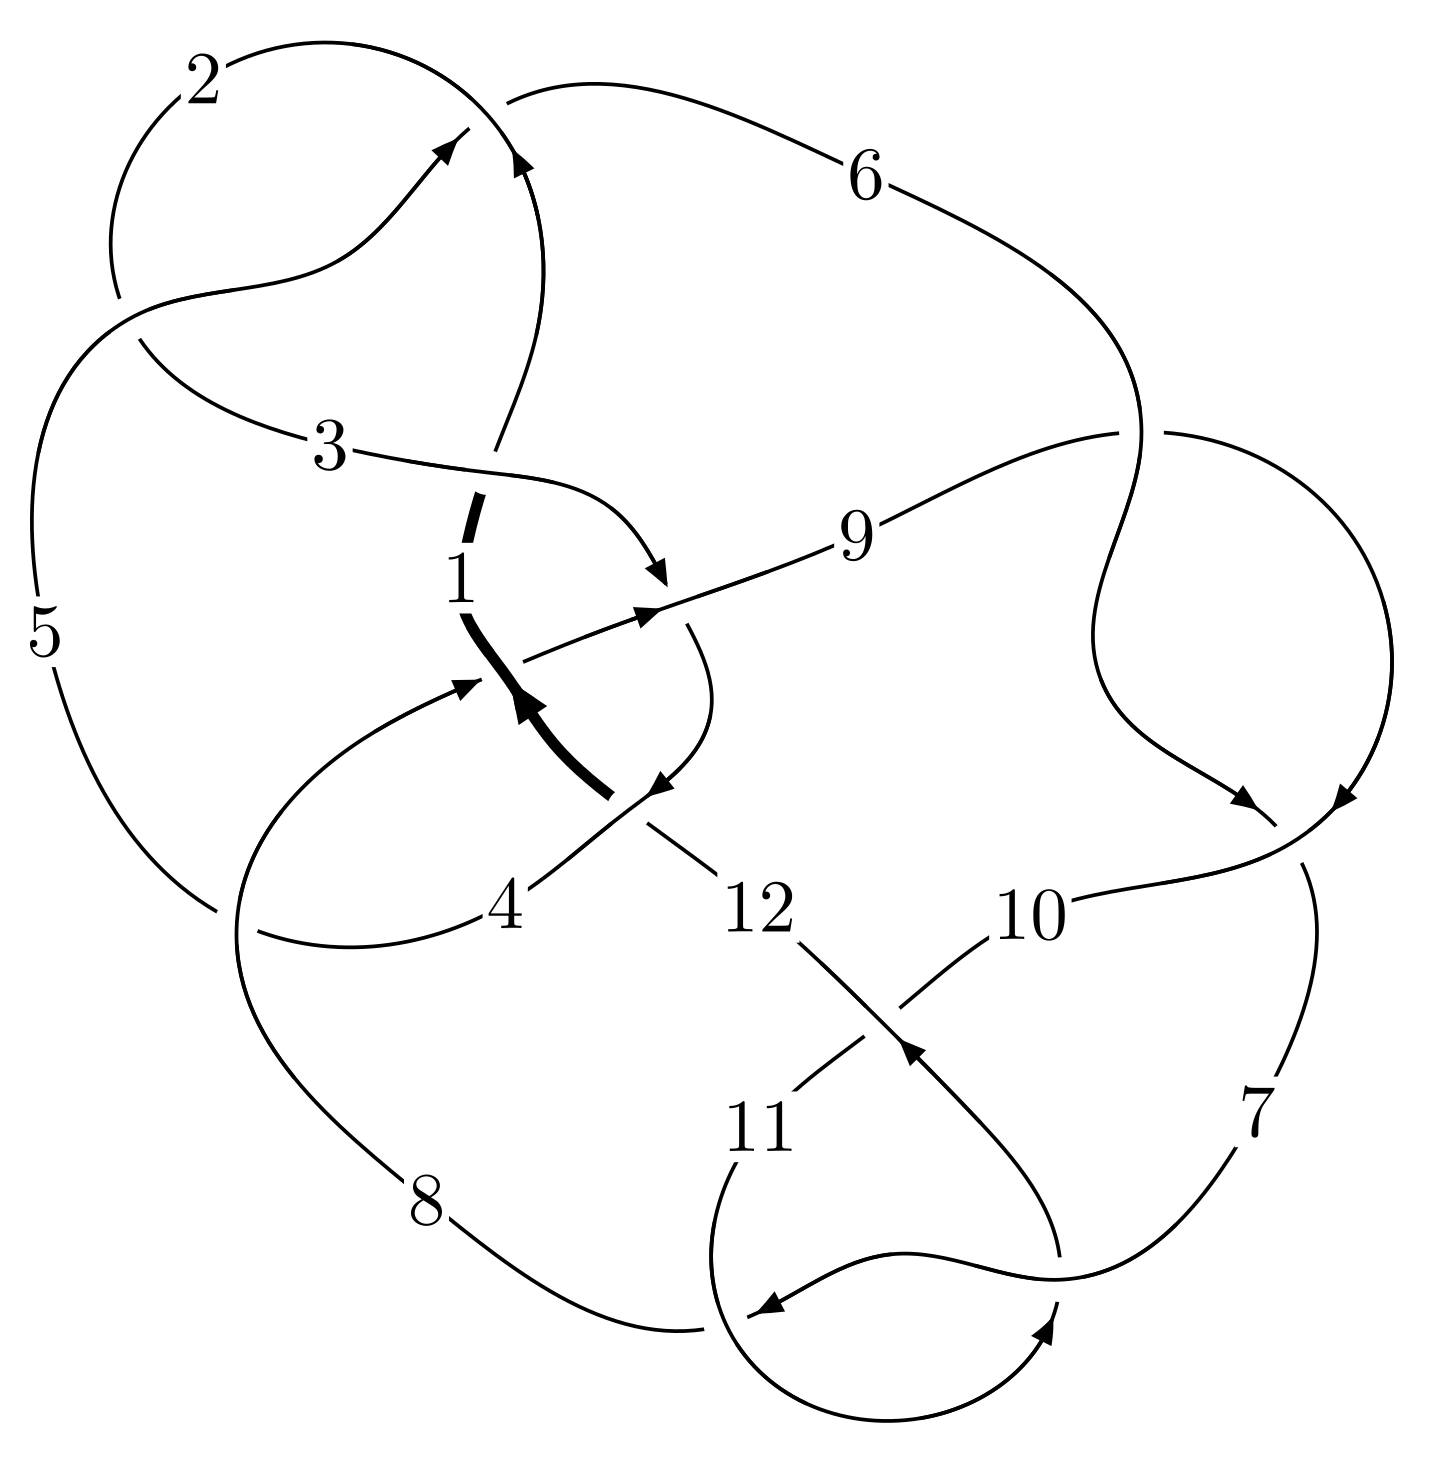
\includegraphics[width=112pt]{../../../GIT/diagram.site/Diagrams/png/990_12a_0189.png}\\
\ \ \ A knot diagram\footnotemark}&
\allowdisplaybreaks
\textbf{Linearized knot diagam} \\
\cline{2-2}
 &
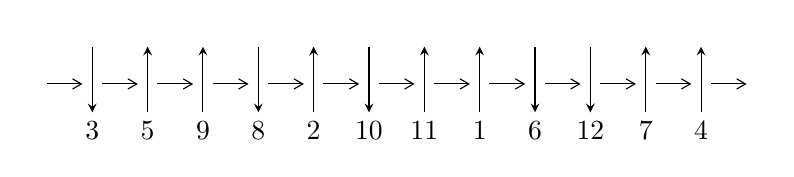
\begin{tikzpicture}[x=20pt, y=17pt]
	% nodes
	\node (C0) at (0, 0) {};
	\node (C1) at (1, 0) {};
	\node (C1U) at (1, +1) {};
	\node (C1D) at (1, -1) {3};

	\node (C2) at (2, 0) {};
	\node (C2U) at (2, +1) {};
	\node (C2D) at (2, -1) {5};

	\node (C3) at (3, 0) {};
	\node (C3U) at (3, +1) {};
	\node (C3D) at (3, -1) {9};

	\node (C4) at (4, 0) {};
	\node (C4U) at (4, +1) {};
	\node (C4D) at (4, -1) {8};

	\node (C5) at (5, 0) {};
	\node (C5U) at (5, +1) {};
	\node (C5D) at (5, -1) {2};

	\node (C6) at (6, 0) {};
	\node (C6U) at (6, +1) {};
	\node (C6D) at (6, -1) {10};

	\node (C7) at (7, 0) {};
	\node (C7U) at (7, +1) {};
	\node (C7D) at (7, -1) {11};

	\node (C8) at (8, 0) {};
	\node (C8U) at (8, +1) {};
	\node (C8D) at (8, -1) {1};

	\node (C9) at (9, 0) {};
	\node (C9U) at (9, +1) {};
	\node (C9D) at (9, -1) {6};

	\node (C10) at (10, 0) {};
	\node (C10U) at (10, +1) {};
	\node (C10D) at (10, -1) {12};

	\node (C11) at (11, 0) {};
	\node (C11U) at (11, +1) {};
	\node (C11D) at (11, -1) {7};

	\node (C12) at (12, 0) {};
	\node (C12U) at (12, +1) {};
	\node (C12D) at (12, -1) {4};
	\node (C13) at (13, 0) {};

	% arrows
	\draw[->,>={angle 60}]
	(C0) edge (C1) (C1) edge (C2) (C2) edge (C3) (C3) edge (C4) (C4) edge (C5) (C5) edge (C6) (C6) edge (C7) (C7) edge (C8) (C8) edge (C9) (C9) edge (C10) (C10) edge (C11) (C11) edge (C12) (C12) edge (C13) ;	\draw[->,>=stealth]
	(C1U) edge (C1D) (C2D) edge (C2U) (C3D) edge (C3U) (C4U) edge (C4D) (C5D) edge (C5U) (C6U) edge (C6D) (C7D) edge (C7U) (C8D) edge (C8U) (C9U) edge (C9D) (C10U) edge (C10D) (C11D) edge (C11U) (C12D) edge (C12U) ;
	\end{tikzpicture} \\
\hhline{~~} \\& 
\textbf{Solving Sequence} \\ \cline{2-2} 
 &
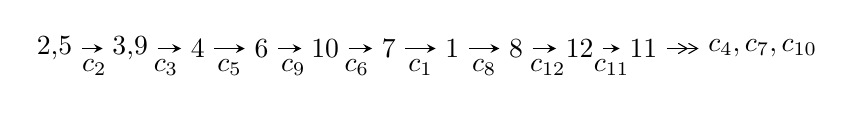
\begin{tikzpicture}[x=23pt, y=7pt]
	% node
	\node (A0) at (-1/8, 0) {2,5};
	\node (A1) at (17/16, 0) {3,9};
	\node (A2) at (17/8, 0) {4};
	\node (A3) at (25/8, 0) {6};
	\node (A4) at (33/8, 0) {10};
	\node (A5) at (41/8, 0) {7};
	\node (A6) at (49/8, 0) {1};
	\node (A7) at (57/8, 0) {8};
	\node (A8) at (65/8, 0) {12};
	\node (A9) at (73/8, 0) {11};
	\node (C1) at (1/2, -1) {$c_{2}$};
	\node (C2) at (13/8, -1) {$c_{3}$};
	\node (C3) at (21/8, -1) {$c_{5}$};
	\node (C4) at (29/8, -1) {$c_{9}$};
	\node (C5) at (37/8, -1) {$c_{6}$};
	\node (C6) at (45/8, -1) {$c_{1}$};
	\node (C7) at (53/8, -1) {$c_{8}$};
	\node (C8) at (61/8, -1) {$c_{12}$};
	\node (C9) at (69/8, -1) {$c_{11}$};
	\node (A10) at (11, 0) {$c_{4},c_{7},c_{10}$};

	% edge
	\draw[->,>=stealth]	
	(A0) edge (A1) (A1) edge (A2) (A2) edge (A3) (A3) edge (A4) (A4) edge (A5) (A5) edge (A6) (A6) edge (A7) (A7) edge (A8) (A8) edge (A9) ;
	\draw[->>,>={angle 60}]	
	(A9) edge (A10);
\end{tikzpicture} \\ 

\end{tabular} \\

\footnotetext{
The image of knot diagram is generated by the software ``\textbf{Draw programme}" developed by Andrew Bartholomew(\url{http://www.layer8.co.uk/maths/draw/index.htm\#Running-draw}), where we modified some parts for our purpose(\url{https://github.com/CATsTAILs/LinksPainter}).
}\phantom \\ \newline 
\centering \textbf{Ideals for irreducible components\footnotemark of $X_{\text{par}}$} 
 
\begin{align*}
I^u_{1}&=\langle 
9.58442\times10^{202} u^{115}-4.19364\times10^{203} u^{114}+\cdots+1.60073\times10^{204} b+2.97710\times10^{203},\\
\phantom{I^u_{1}}&\phantom{= \langle  }7.26221\times10^{203} u^{115}-2.06580\times10^{204} u^{114}+\cdots+8.00367\times10^{203} a-3.78417\times10^{204},\;u^{116}-3 u^{115}+\cdots+2 u+1\rangle \\
I^u_{2}&=\langle 
b+2 u+2,\;a+u+2,\;u^2+u+1\rangle \\
I^u_{3}&=\langle 
b- u-1,\;a- u-2,\;u^2+u+1\rangle \\
\\
\end{align*}
\raggedright * 3 irreducible components of $\dim_{\mathbb{C}}=0$, with total 120 representations.\\
\footnotetext{All coefficients of polynomials are rational numbers. But the coefficients are sometimes approximated in decimal forms when there is not enough margin.}
\newpage
\renewcommand{\arraystretch}{1}
\centering \section*{I. $I^u_{1}= \langle 9.58\times10^{202} u^{115}-4.19\times10^{203} u^{114}+\cdots+1.60\times10^{204} b+2.98\times10^{203},\;7.26\times10^{203} u^{115}-2.07\times10^{204} u^{114}+\cdots+8.00\times10^{203} a-3.78\times10^{204},\;u^{116}-3 u^{115}+\cdots+2 u+1 \rangle$}
\flushleft \textbf{(i) Arc colorings}\\
\begin{tabular}{m{7pt} m{180pt} m{7pt} m{180pt} }
\flushright $a_{2}=$&$\begin{pmatrix}1\\0\end{pmatrix}$ \\
\flushright $a_{5}=$&$\begin{pmatrix}0\\u\end{pmatrix}$ \\
\flushright $a_{3}=$&$\begin{pmatrix}1\\- u^2\end{pmatrix}$ \\
\flushright $a_{9}=$&$\begin{pmatrix}-0.907360 u^{115}+2.58106 u^{114}+\cdots-44.6961 u+4.72805\\-0.0598752 u^{115}+0.261982 u^{114}+\cdots-4.69798 u-0.185983\end{pmatrix}$ \\
\flushright $a_{4}=$&$\begin{pmatrix}0.373553 u^{115}-1.05557 u^{114}+\cdots+3.05131 u+4.40925\\-0.0574361 u^{115}+0.427091 u^{114}+\cdots-0.705757 u+0.556895\end{pmatrix}$ \\
\flushright $a_{6}=$&$\begin{pmatrix}u\\u\end{pmatrix}$ \\
\flushright $a_{10}=$&$\begin{pmatrix}-0.579574 u^{115}+2.08631 u^{114}+\cdots-43.4018 u+4.95142\\0.267911 u^{115}-0.232768 u^{114}+\cdots-3.40374 u+0.0373916\end{pmatrix}$ \\
\flushright $a_{7}=$&$\begin{pmatrix}-0.347099 u^{115}+0.843729 u^{114}+\cdots+0.329330 u-4.71183\\-0.978083 u^{115}+2.09051 u^{114}+\cdots+2.73850 u-0.265630\end{pmatrix}$ \\
\flushright $a_{1}=$&$\begin{pmatrix}u^2+1\\- u^4\end{pmatrix}$ \\
\flushright $a_{8}=$&$\begin{pmatrix}-0.609059 u^{115}+1.74035 u^{114}+\cdots-39.7192 u+4.90364\\0.472186 u^{115}-1.17053 u^{114}+\cdots-5.34613 u-0.562955\end{pmatrix}$ \\
\flushright $a_{12}=$&$\begin{pmatrix}0.0341312 u^{115}-0.0138481 u^{114}+\cdots-4.87772 u+2.57110\\0.171988 u^{115}-0.197880 u^{114}+\cdots-0.274653 u+0.227357\end{pmatrix}$ \\
\flushright $a_{11}=$&$\begin{pmatrix}-0.0990931 u^{115}+0.174632 u^{114}+\cdots-38.4334 u+4.70463\\-1.61684 u^{115}+2.77771 u^{114}+\cdots-6.68015 u-0.578114\end{pmatrix}$\\&\end{tabular}
\flushleft \textbf{(ii) Obstruction class $= -1$}\\~\\
\flushleft \textbf{(iii) Cusp Shapes $= 2.83036 u^{115}-6.91712 u^{114}+\cdots+32.6663 u-0.776136$}\\~\\
\newpage\renewcommand{\arraystretch}{1}
\flushleft \textbf{(iv) u-Polynomials at the component}\newline \\
\begin{tabular}{m{50pt}|m{274pt}}
Crossings & \hspace{64pt}u-Polynomials at each crossing \\
\hline $$\begin{aligned}c_{1}\end{aligned}$$&$\begin{aligned}
&u^{116}+51 u^{115}+\cdots+90 u+1
\end{aligned}$\\
\hline $$\begin{aligned}c_{2},c_{5}\end{aligned}$$&$\begin{aligned}
&u^{116}+3 u^{115}+\cdots-2 u+1
\end{aligned}$\\
\hline $$\begin{aligned}c_{3}\end{aligned}$$&$\begin{aligned}
&u^{116}-56 u^{114}+\cdots-1192 u+608
\end{aligned}$\\
\hline $$\begin{aligned}c_{4}\end{aligned}$$&$\begin{aligned}
&u^{116}+2 u^{115}+\cdots-20233 u-2189
\end{aligned}$\\
\hline $$\begin{aligned}c_{6},c_{9}\end{aligned}$$&$\begin{aligned}
&u^{116}+3 u^{115}+\cdots+493 u+578
\end{aligned}$\\
\hline $$\begin{aligned}c_{7},c_{11}\end{aligned}$$&$\begin{aligned}
&u^{116}-3 u^{115}+\cdots-8 u+1
\end{aligned}$\\
\hline $$\begin{aligned}c_{8}\end{aligned}$$&$\begin{aligned}
&u^{116}-3 u^{115}+\cdots-2 u+1
\end{aligned}$\\
\hline $$\begin{aligned}c_{10}\end{aligned}$$&$\begin{aligned}
&u^{116}+63 u^{115}+\cdots-2 u+1
\end{aligned}$\\
\hline $$\begin{aligned}c_{12}\end{aligned}$$&$\begin{aligned}
&u^{116}+11 u^{115}+\cdots+48 u+16
\end{aligned}$\\
\hline
\end{tabular}\\~\\
\newpage\renewcommand{\arraystretch}{1}
\flushleft \textbf{(v) Riley Polynomials at the component}\newline \\
\begin{tabular}{m{50pt}|m{274pt}}
Crossings & \hspace{64pt}Riley Polynomials at each crossing \\
\hline $$\begin{aligned}c_{1}\end{aligned}$$&$\begin{aligned}
&y^{116}+31 y^{115}+\cdots+9626 y+1
\end{aligned}$\\
\hline $$\begin{aligned}c_{2},c_{5}\end{aligned}$$&$\begin{aligned}
&y^{116}+51 y^{115}+\cdots+90 y+1
\end{aligned}$\\
\hline $$\begin{aligned}c_{3}\end{aligned}$$&$\begin{aligned}
&y^{116}-112 y^{115}+\cdots+12874432 y+369664
\end{aligned}$\\
\hline $$\begin{aligned}c_{4}\end{aligned}$$&$\begin{aligned}
&y^{116}-140 y^{115}+\cdots-610858605 y+4791721
\end{aligned}$\\
\hline $$\begin{aligned}c_{6},c_{9}\end{aligned}$$&$\begin{aligned}
&y^{116}-97 y^{115}+\cdots+5595907 y+334084
\end{aligned}$\\
\hline $$\begin{aligned}c_{7},c_{11}\end{aligned}$$&$\begin{aligned}
&y^{116}+63 y^{115}+\cdots-2 y+1
\end{aligned}$\\
\hline $$\begin{aligned}c_{8}\end{aligned}$$&$\begin{aligned}
&y^{116}-9 y^{115}+\cdots-2 y+1
\end{aligned}$\\
\hline $$\begin{aligned}c_{10}\end{aligned}$$&$\begin{aligned}
&y^{116}-17 y^{115}+\cdots+154 y+1
\end{aligned}$\\
\hline $$\begin{aligned}c_{12}\end{aligned}$$&$\begin{aligned}
&y^{116}+25 y^{115}+\cdots+7552 y+256
\end{aligned}$\\
\hline
\end{tabular}\\~\\
\newpage\flushleft \textbf{(vi) Complex Volumes and Cusp Shapes}
$$\begin{array}{c|c|c}  
\text{Solutions to }I^u_{1}& \I (\text{vol} + \sqrt{-1}CS) & \text{Cusp shape}\\
 \hline 
\begin{aligned}
u &= -0.999176 + 0.073817 I \\
a &= -1.158200 + 0.036546 I \\
b &= \phantom{-}0.186255 - 0.167090 I\end{aligned}
 & -2.03780 + 4.18277 I & \phantom{-0.000000 } 0 \\ \hline\begin{aligned}
u &= -0.999176 - 0.073817 I \\
a &= -1.158200 - 0.036546 I \\
b &= \phantom{-}0.186255 + 0.167090 I\end{aligned}
 & -2.03780 - 4.18277 I & \phantom{-0.000000 } 0 \\ \hline\begin{aligned}
u &= \phantom{-}0.920845 + 0.376102 I \\
a &= \phantom{-}0.83921 - 1.20374 I \\
b &= -0.413762 - 0.802174 I\end{aligned}
 & -5.71061 - 3.88667 I & \phantom{-0.000000 } 0 \\ \hline\begin{aligned}
u &= \phantom{-}0.920845 - 0.376102 I \\
a &= \phantom{-}0.83921 + 1.20374 I \\
b &= -0.413762 + 0.802174 I\end{aligned}
 & -5.71061 + 3.88667 I & \phantom{-0.000000 } 0 \\ \hline\begin{aligned}
u &= \phantom{-}0.924268 + 0.411448 I \\
a &= -0.94680 + 1.15560 I \\
b &= \phantom{-}0.460141 + 0.963298 I\end{aligned}
 & -1.55371 - 8.03241 I & \phantom{-0.000000 } 0 \\ \hline\begin{aligned}
u &= \phantom{-}0.924268 - 0.411448 I \\
a &= -0.94680 - 1.15560 I \\
b &= \phantom{-}0.460141 - 0.963298 I\end{aligned}
 & -1.55371 + 8.03241 I & \phantom{-0.000000 } 0 \\ \hline\begin{aligned}
u &= \phantom{-}0.421700 + 0.925453 I \\
a &= -1.92345 + 0.70480 I \\
b &= -0.97816 + 1.68161 I\end{aligned}
 & -0.71802 + 4.11793 I & \phantom{-0.000000 } 0 \\ \hline\begin{aligned}
u &= \phantom{-}0.421700 - 0.925453 I \\
a &= -1.92345 - 0.70480 I \\
b &= -0.97816 - 1.68161 I\end{aligned}
 & -0.71802 - 4.11793 I & \phantom{-0.000000 } 0 \\ \hline\begin{aligned}
u &= -0.514672 + 0.835355 I \\
a &= -2.38620 - 2.63903 I \\
b &= -1.70821 - 2.74409 I\end{aligned}
 & -0.071703 - 0.449560 I & \phantom{-0.000000 } 0 \\ \hline\begin{aligned}
u &= -0.514672 - 0.835355 I \\
a &= -2.38620 + 2.63903 I \\
b &= -1.70821 + 2.74409 I\end{aligned}
 & -0.071703 + 0.449560 I & \phantom{-0.000000 } 0\\
 \hline 
 \end{array}$$\newpage$$\begin{array}{c|c|c}  
\text{Solutions to }I^u_{1}& \I (\text{vol} + \sqrt{-1}CS) & \text{Cusp shape}\\
 \hline 
\begin{aligned}
u &= -0.522133 + 0.877863 I \\
a &= \phantom{-}2.24240 + 2.97424 I \\
b &= \phantom{-}1.90261 + 3.57304 I\end{aligned}
 & -0.21332 - 3.74883 I & \phantom{-0.000000 } 0 \\ \hline\begin{aligned}
u &= -0.522133 - 0.877863 I \\
a &= \phantom{-}2.24240 - 2.97424 I \\
b &= \phantom{-}1.90261 - 3.57304 I\end{aligned}
 & -0.21332 + 3.74883 I & \phantom{-0.000000 } 0 \\ \hline\begin{aligned}
u &= \phantom{-}0.839409 + 0.494565 I \\
a &= -1.045040 + 0.780335 I \\
b &= \phantom{-}0.067833 + 1.333700 I\end{aligned}
 & \phantom{-}2.46054 - 7.61264 I & \phantom{-0.000000 } 0 \\ \hline\begin{aligned}
u &= \phantom{-}0.839409 - 0.494565 I \\
a &= -1.045040 - 0.780335 I \\
b &= \phantom{-}0.067833 - 1.333700 I\end{aligned}
 & \phantom{-}2.46054 + 7.61264 I & \phantom{-0.000000 } 0 \\ \hline\begin{aligned}
u &= -0.878140 + 0.408645 I \\
a &= \phantom{-}0.852110 - 0.076165 I \\
b &= \phantom{-}0.325025 + 0.552285 I\end{aligned}
 & \phantom{-}2.68929 + 0.25500 I & \phantom{-0.000000 } 0 \\ \hline\begin{aligned}
u &= -0.878140 - 0.408645 I \\
a &= \phantom{-}0.852110 + 0.076165 I \\
b &= \phantom{-}0.325025 - 0.552285 I\end{aligned}
 & \phantom{-}2.68929 - 0.25500 I & \phantom{-0.000000 } 0 \\ \hline\begin{aligned}
u &= \phantom{-}0.948659 + 0.414465 I \\
a &= \phantom{-}0.99590 - 1.22076 I \\
b &= -0.583121 - 0.960239 I\end{aligned}
 & -4.76188 - 12.96690 I & \phantom{-0.000000 } 0 \\ \hline\begin{aligned}
u &= \phantom{-}0.948659 - 0.414465 I \\
a &= \phantom{-}0.99590 + 1.22076 I \\
b &= -0.583121 + 0.960239 I\end{aligned}
 & -4.76188 + 12.96690 I & \phantom{-0.000000 } 0 \\ \hline\begin{aligned}
u &= -0.006481 + 0.960054 I \\
a &= \phantom{-}0.396095 - 1.053930 I \\
b &= -0.177120 - 0.492167 I\end{aligned}
 & -1.96858 - 1.97750 I & \phantom{-0.000000 } 0 \\ \hline\begin{aligned}
u &= -0.006481 - 0.960054 I \\
a &= \phantom{-}0.396095 + 1.053930 I \\
b &= -0.177120 + 0.492167 I\end{aligned}
 & -1.96858 + 1.97750 I & \phantom{-0.000000 } 0\\
 \hline 
 \end{array}$$\newpage$$\begin{array}{c|c|c}  
\text{Solutions to }I^u_{1}& \I (\text{vol} + \sqrt{-1}CS) & \text{Cusp shape}\\
 \hline 
\begin{aligned}
u &= -0.898263 + 0.550730 I \\
a &= -0.646075 + 0.173708 I \\
b &= -0.505703 - 0.604282 I\end{aligned}
 & \phantom{-}2.55387 - 3.56596 I & \phantom{-0.000000 } 0 \\ \hline\begin{aligned}
u &= -0.898263 - 0.550730 I \\
a &= -0.646075 - 0.173708 I \\
b &= -0.505703 + 0.604282 I\end{aligned}
 & \phantom{-}2.55387 + 3.56596 I & \phantom{-0.000000 } 0 \\ \hline\begin{aligned}
u &= -0.486090 + 0.945475 I \\
a &= \phantom{-}1.95773 + 2.14041 I \\
b &= \phantom{-}2.41861 + 3.20916 I\end{aligned}
 & -2.64076 - 2.51596 I & \phantom{-0.000000 } 0 \\ \hline\begin{aligned}
u &= -0.486090 - 0.945475 I \\
a &= \phantom{-}1.95773 - 2.14041 I \\
b &= \phantom{-}2.41861 - 3.20916 I\end{aligned}
 & -2.64076 + 2.51596 I & \phantom{-0.000000 } 0 \\ \hline\begin{aligned}
u &= \phantom{-}0.302821 + 1.020470 I \\
a &= \phantom{-}0.129693 + 0.508484 I \\
b &= \phantom{-}0.787123 - 0.928929 I\end{aligned}
 & -9.27722 - 3.99137 I & \phantom{-0.000000 } 0 \\ \hline\begin{aligned}
u &= \phantom{-}0.302821 - 1.020470 I \\
a &= \phantom{-}0.129693 - 0.508484 I \\
b &= \phantom{-}0.787123 + 0.928929 I\end{aligned}
 & -9.27722 + 3.99137 I & \phantom{-0.000000 } 0 \\ \hline\begin{aligned}
u &= \phantom{-}0.776802 + 0.518793 I \\
a &= \phantom{-}1.015560 - 0.567370 I \\
b &= \phantom{-}0.204586 - 1.364390 I\end{aligned}
 & \phantom{-}3.39422 - 3.00637 I & \phantom{-0.000000 } 0 \\ \hline\begin{aligned}
u &= \phantom{-}0.776802 - 0.518793 I \\
a &= \phantom{-}1.015560 + 0.567370 I \\
b &= \phantom{-}0.204586 + 1.364390 I\end{aligned}
 & \phantom{-}3.39422 + 3.00637 I & \phantom{-0.000000 } 0 \\ \hline\begin{aligned}
u &= \phantom{-}0.359469 + 0.860704 I \\
a &= \phantom{-}1.66643 - 1.09222 I \\
b &= \phantom{-}0.41232 - 1.47680 I\end{aligned}
 & -0.359640 - 0.841106 I & \phantom{-0.000000 } 0 \\ \hline\begin{aligned}
u &= \phantom{-}0.359469 - 0.860704 I \\
a &= \phantom{-}1.66643 + 1.09222 I \\
b &= \phantom{-}0.41232 + 1.47680 I\end{aligned}
 & -0.359640 + 0.841106 I & \phantom{-0.000000 } 0\\
 \hline 
 \end{array}$$\newpage$$\begin{array}{c|c|c}  
\text{Solutions to }I^u_{1}& \I (\text{vol} + \sqrt{-1}CS) & \text{Cusp shape}\\
 \hline 
\begin{aligned}
u &= \phantom{-}0.344814 + 1.011520 I \\
a &= -0.014959 - 0.630159 I \\
b &= -0.674659 + 0.692719 I\end{aligned}
 & -5.70935 + 0.95306 I & \phantom{-0.000000 } 0 \\ \hline\begin{aligned}
u &= \phantom{-}0.344814 - 1.011520 I \\
a &= -0.014959 + 0.630159 I \\
b &= -0.674659 - 0.692719 I\end{aligned}
 & -5.70935 - 0.95306 I & \phantom{-0.000000 } 0 \\ \hline\begin{aligned}
u &= -0.469947 + 0.964016 I \\
a &= -1.97650 - 1.92488 I \\
b &= -2.68528 - 3.02412 I\end{aligned}
 & -6.22272 + 1.80974 I & \phantom{-0.000000 } 0 \\ \hline\begin{aligned}
u &= -0.469947 - 0.964016 I \\
a &= -1.97650 + 1.92488 I \\
b &= -2.68528 + 3.02412 I\end{aligned}
 & -6.22272 - 1.80974 I & \phantom{-0.000000 } 0 \\ \hline\begin{aligned}
u &= -0.413064 + 0.829110 I \\
a &= \phantom{-}0.77676 + 1.50532 I \\
b &= \phantom{-}1.30264 + 1.62629 I\end{aligned}
 & -0.811819 - 0.337167 I & \phantom{-0.000000 } 0 \\ \hline\begin{aligned}
u &= -0.413064 - 0.829110 I \\
a &= \phantom{-}0.77676 - 1.50532 I \\
b &= \phantom{-}1.30264 - 1.62629 I\end{aligned}
 & -0.811819 + 0.337167 I & \phantom{-0.000000 } 0 \\ \hline\begin{aligned}
u &= -0.622446 + 0.880279 I \\
a &= \phantom{-}0.568985 - 0.163247 I \\
b &= \phantom{-}0.283062 - 0.213587 I\end{aligned}
 & \phantom{-}0.60755 - 2.45684 I & \phantom{-0.000000 } 0 \\ \hline\begin{aligned}
u &= -0.622446 - 0.880279 I \\
a &= \phantom{-}0.568985 + 0.163247 I \\
b &= \phantom{-}0.283062 + 0.213587 I\end{aligned}
 & \phantom{-}0.60755 + 2.45684 I & \phantom{-0.000000 } 0 \\ \hline\begin{aligned}
u &= -0.503225 + 0.958571 I \\
a &= -2.14933 - 2.14897 I \\
b &= -2.56067 - 3.44707 I\end{aligned}
 & -6.03961 - 7.01535 I & \phantom{-0.000000 } 0 \\ \hline\begin{aligned}
u &= -0.503225 - 0.958571 I \\
a &= -2.14933 + 2.14897 I \\
b &= -2.56067 + 3.44707 I\end{aligned}
 & -6.03961 + 7.01535 I & \phantom{-0.000000 } 0\\
 \hline 
 \end{array}$$\newpage$$\begin{array}{c|c|c}  
\text{Solutions to }I^u_{1}& \I (\text{vol} + \sqrt{-1}CS) & \text{Cusp shape}\\
 \hline 
\begin{aligned}
u &= \phantom{-}0.540140 + 0.972262 I \\
a &= \phantom{-}0.91775 - 1.34992 I \\
b &= -0.382108 - 1.078750 I\end{aligned}
 & \phantom{-}0.159951 + 1.001520 I & \phantom{-0.000000 } 0 \\ \hline\begin{aligned}
u &= \phantom{-}0.540140 - 0.972262 I \\
a &= \phantom{-}0.91775 + 1.34992 I \\
b &= -0.382108 + 1.078750 I\end{aligned}
 & \phantom{-}0.159951 - 1.001520 I & \phantom{-0.000000 } 0 \\ \hline\begin{aligned}
u &= \phantom{-}0.364288 + 1.052870 I \\
a &= -0.152278 + 0.524830 I \\
b &= \phantom{-}0.353280 - 0.740875 I\end{aligned}
 & -9.79216 + 5.52663 I & \phantom{-0.000000 } 0 \\ \hline\begin{aligned}
u &= \phantom{-}0.364288 - 1.052870 I \\
a &= -0.152278 - 0.524830 I \\
b &= \phantom{-}0.353280 + 0.740875 I\end{aligned}
 & -9.79216 - 5.52663 I & \phantom{-0.000000 } 0 \\ \hline\begin{aligned}
u &= \phantom{-}0.216355 + 1.098250 I \\
a &= -0.934801 + 0.417662 I \\
b &= -0.740885 + 0.207706 I\end{aligned}
 & -6.10304 - 0.25139 I & \phantom{-0.000000 } 0 \\ \hline\begin{aligned}
u &= \phantom{-}0.216355 - 1.098250 I \\
a &= -0.934801 - 0.417662 I \\
b &= -0.740885 - 0.207706 I\end{aligned}
 & -6.10304 + 0.25139 I & \phantom{-0.000000 } 0 \\ \hline\begin{aligned}
u &= \phantom{-}0.564834 + 0.664610 I \\
a &= -1.104790 - 0.262157 I \\
b &= -1.10291 + 1.29255 I\end{aligned}
 & \phantom{-}1.11308 + 3.43678 I & \phantom{-0.000000 } 0 \\ \hline\begin{aligned}
u &= \phantom{-}0.564834 - 0.664610 I \\
a &= -1.104790 + 0.262157 I \\
b &= -1.10291 - 1.29255 I\end{aligned}
 & \phantom{-}1.11308 - 3.43678 I & \phantom{-0.000000 } 0 \\ \hline\begin{aligned}
u &= -0.864925\phantom{ +0.000000I} \\
a &= \phantom{-}1.12947\phantom{ +0.000000I} \\
b &= \phantom{-}0.0590391\phantom{ +0.000000I}\end{aligned}
 & \phantom{-}1.15090\phantom{ +0.000000I} & \phantom{-0.000000 } 0 \\ \hline\begin{aligned}
u &= \phantom{-}0.634001 + 0.579385 I \\
a &= \phantom{-}0.972987 - 0.075164 I \\
b &= \phantom{-}0.73859 - 1.29757 I\end{aligned}
 & \phantom{-}2.80840 - 1.23277 I & \phantom{-0.000000 } 0\\
 \hline 
 \end{array}$$\newpage$$\begin{array}{c|c|c}  
\text{Solutions to }I^u_{1}& \I (\text{vol} + \sqrt{-1}CS) & \text{Cusp shape}\\
 \hline 
\begin{aligned}
u &= \phantom{-}0.634001 - 0.579385 I \\
a &= \phantom{-}0.972987 + 0.075164 I \\
b &= \phantom{-}0.73859 + 1.29757 I\end{aligned}
 & \phantom{-}2.80840 + 1.23277 I & \phantom{-0.000000 } 0 \\ \hline\begin{aligned}
u &= -0.424391 + 1.064250 I \\
a &= -0.804446 - 0.658783 I \\
b &= -1.053830 - 0.611339 I\end{aligned}
 & -1.61821 - 2.77049 I & \phantom{-0.000000 } 0 \\ \hline\begin{aligned}
u &= -0.424391 - 1.064250 I \\
a &= -0.804446 + 0.658783 I \\
b &= -1.053830 + 0.611339 I\end{aligned}
 & -1.61821 + 2.77049 I & \phantom{-0.000000 } 0 \\ \hline\begin{aligned}
u &= \phantom{-}0.496996 + 1.048050 I \\
a &= -1.78524 + 0.10263 I \\
b &= -1.89932 + 1.40555 I\end{aligned}
 & -4.68200 + 5.54586 I & \phantom{-0.000000 } 0 \\ \hline\begin{aligned}
u &= \phantom{-}0.496996 - 1.048050 I \\
a &= -1.78524 - 0.10263 I \\
b &= -1.89932 - 1.40555 I\end{aligned}
 & -4.68200 - 5.54586 I & \phantom{-0.000000 } 0 \\ \hline\begin{aligned}
u &= \phantom{-}0.576297 + 1.006970 I \\
a &= -1.14686 + 1.15350 I \\
b &= -0.082280 + 1.271190 I\end{aligned}
 & \phantom{-}1.53237 + 5.99820 I & \phantom{-0.000000 } 0 \\ \hline\begin{aligned}
u &= \phantom{-}0.576297 - 1.006970 I \\
a &= -1.14686 - 1.15350 I \\
b &= -0.082280 - 1.271190 I\end{aligned}
 & \phantom{-}1.53237 - 5.99820 I & \phantom{-0.000000 } 0 \\ \hline\begin{aligned}
u &= -0.495476 + 0.676963 I \\
a &= \phantom{-}1.35903 + 3.12852 I \\
b &= \phantom{-}0.14569 + 2.00460 I\end{aligned}
 & -5.17764 + 2.89665 I & \phantom{-0.000000 } 0 \\ \hline\begin{aligned}
u &= -0.495476 - 0.676963 I \\
a &= \phantom{-}1.35903 - 3.12852 I \\
b &= \phantom{-}0.14569 - 2.00460 I\end{aligned}
 & -5.17764 - 2.89665 I & \phantom{-0.000000 } 0 \\ \hline\begin{aligned}
u &= -0.054161 + 1.167310 I \\
a &= -0.098432 + 0.478297 I \\
b &= \phantom{-}0.446919 - 0.165131 I\end{aligned}
 & -3.65497 - 5.87029 I & \phantom{-0.000000 } 0\\
 \hline 
 \end{array}$$\newpage$$\begin{array}{c|c|c}  
\text{Solutions to }I^u_{1}& \I (\text{vol} + \sqrt{-1}CS) & \text{Cusp shape}\\
 \hline 
\begin{aligned}
u &= -0.054161 - 1.167310 I \\
a &= -0.098432 - 0.478297 I \\
b &= \phantom{-}0.446919 + 0.165131 I\end{aligned}
 & -3.65497 + 5.87029 I & \phantom{-0.000000 } 0 \\ \hline\begin{aligned}
u &= \phantom{-}0.469726 + 1.082720 I \\
a &= \phantom{-}1.66244 - 0.08554 I \\
b &= \phantom{-}1.92404 - 1.13006 I\end{aligned}
 & -9.06972 + 1.47220 I & \phantom{-0.000000 } 0 \\ \hline\begin{aligned}
u &= \phantom{-}0.469726 - 1.082720 I \\
a &= \phantom{-}1.66244 + 0.08554 I \\
b &= \phantom{-}1.92404 + 1.13006 I\end{aligned}
 & -9.06972 - 1.47220 I & \phantom{-0.000000 } 0 \\ \hline\begin{aligned}
u &= -0.424271 + 0.698754 I \\
a &= -1.09326 - 2.76432 I \\
b &= -0.39351 - 1.66424 I\end{aligned}
 & -1.86322 - 1.38201 I & \phantom{-0.000000 } 0 \\ \hline\begin{aligned}
u &= -0.424271 - 0.698754 I \\
a &= -1.09326 + 2.76432 I \\
b &= -0.39351 + 1.66424 I\end{aligned}
 & -1.86322 + 1.38201 I & \phantom{-0.000000 } 0 \\ \hline\begin{aligned}
u &= \phantom{-}0.523478 + 1.060820 I \\
a &= \phantom{-}1.80466 - 0.02934 I \\
b &= \phantom{-}2.06619 - 1.46486 I\end{aligned}
 & -7.81039 + 10.63470 I & \phantom{-0.000000 } 0 \\ \hline\begin{aligned}
u &= \phantom{-}0.523478 - 1.060820 I \\
a &= \phantom{-}1.80466 + 0.02934 I \\
b &= \phantom{-}2.06619 + 1.46486 I\end{aligned}
 & -7.81039 - 10.63470 I & \phantom{-0.000000 } 0 \\ \hline\begin{aligned}
u &= -0.912005 + 0.778203 I \\
a &= -0.223087 + 0.395516 I \\
b &= -0.815991 - 0.278111 I\end{aligned}
 & \phantom{-}0.41964 - 3.21534 I & \phantom{-0.000000 } 0 \\ \hline\begin{aligned}
u &= -0.912005 - 0.778203 I \\
a &= -0.223087 - 0.395516 I \\
b &= -0.815991 + 0.278111 I\end{aligned}
 & \phantom{-}0.41964 + 3.21534 I & \phantom{-0.000000 } 0 \\ \hline\begin{aligned}
u &= \phantom{-}0.557526 + 1.084810 I \\
a &= \phantom{-}1.122080 - 0.735761 I \\
b &= \phantom{-}0.780432 - 0.806136 I\end{aligned}
 & -3.94544 + 7.44938 I & \phantom{-0.000000 } 0\\
 \hline 
 \end{array}$$\newpage$$\begin{array}{c|c|c}  
\text{Solutions to }I^u_{1}& \I (\text{vol} + \sqrt{-1}CS) & \text{Cusp shape}\\
 \hline 
\begin{aligned}
u &= \phantom{-}0.557526 - 1.084810 I \\
a &= \phantom{-}1.122080 + 0.735761 I \\
b &= \phantom{-}0.780432 + 0.806136 I\end{aligned}
 & -3.94544 - 7.44938 I & \phantom{-0.000000 } 0 \\ \hline\begin{aligned}
u &= \phantom{-}0.628411 + 1.064180 I \\
a &= -1.43841 + 0.90795 I \\
b &= -0.79030 + 1.61396 I\end{aligned}
 & \phantom{-}1.75781 + 8.31581 I & \phantom{-0.000000 } 0 \\ \hline\begin{aligned}
u &= \phantom{-}0.628411 - 1.064180 I \\
a &= -1.43841 - 0.90795 I \\
b &= -0.79030 - 1.61396 I\end{aligned}
 & \phantom{-}1.75781 - 8.31581 I & \phantom{-0.000000 } 0 \\ \hline\begin{aligned}
u &= -0.713776 + 1.019460 I \\
a &= \phantom{-}0.535297 + 0.394961 I \\
b &= \phantom{-}0.061365 + 0.653781 I\end{aligned}
 & \phantom{-}1.16025 - 2.35383 I & \phantom{-0.000000 } 0 \\ \hline\begin{aligned}
u &= -0.713776 - 1.019460 I \\
a &= \phantom{-}0.535297 - 0.394961 I \\
b &= \phantom{-}0.061365 - 0.653781 I\end{aligned}
 & \phantom{-}1.16025 + 2.35383 I & \phantom{-0.000000 } 0 \\ \hline\begin{aligned}
u &= -0.976305 + 0.778911 I \\
a &= \phantom{-}0.294860 - 0.522815 I \\
b &= \phantom{-}1.004610 + 0.376001 I\end{aligned}
 & -2.76590 - 7.61812 I & \phantom{-0.000000 } 0 \\ \hline\begin{aligned}
u &= -0.976305 - 0.778911 I \\
a &= \phantom{-}0.294860 + 0.522815 I \\
b &= \phantom{-}1.004610 - 0.376001 I\end{aligned}
 & -2.76590 + 7.61812 I & \phantom{-0.000000 } 0 \\ \hline\begin{aligned}
u &= \phantom{-}0.661618 + 0.345676 I \\
a &= -0.343334 + 0.497854 I \\
b &= -0.413165 + 0.801179 I\end{aligned}
 & -1.87219 - 2.71430 I & -2.15624 + 3.40858 I \\ \hline\begin{aligned}
u &= \phantom{-}0.661618 - 0.345676 I \\
a &= -0.343334 - 0.497854 I \\
b &= -0.413165 - 0.801179 I\end{aligned}
 & -1.87219 + 2.71430 I & -2.15624 - 3.40858 I \\ \hline\begin{aligned}
u &= -0.930176 + 0.855473 I \\
a &= \phantom{-}0.090059 - 0.524656 I \\
b &= \phantom{-}0.967564 + 0.038882 I\end{aligned}
 & -3.00978 + 0.86920 I & \phantom{-0.000000 } 0\\
 \hline 
 \end{array}$$\newpage$$\begin{array}{c|c|c}  
\text{Solutions to }I^u_{1}& \I (\text{vol} + \sqrt{-1}CS) & \text{Cusp shape}\\
 \hline 
\begin{aligned}
u &= -0.930176 - 0.855473 I \\
a &= \phantom{-}0.090059 + 0.524656 I \\
b &= \phantom{-}0.967564 - 0.038882 I\end{aligned}
 & -3.00978 - 0.86920 I & \phantom{-0.000000 } 0 \\ \hline\begin{aligned}
u &= \phantom{-}0.647248 + 1.091120 I \\
a &= \phantom{-}1.54881 - 0.80607 I \\
b &= \phantom{-}1.12488 - 1.75934 I\end{aligned}
 & \phantom{-}0.65942 + 13.14560 I & \phantom{-0.000000 } 0 \\ \hline\begin{aligned}
u &= \phantom{-}0.647248 - 1.091120 I \\
a &= \phantom{-}1.54881 + 0.80607 I \\
b &= \phantom{-}1.12488 + 1.75934 I\end{aligned}
 & \phantom{-}0.65942 - 13.14560 I & \phantom{-0.000000 } 0 \\ \hline\begin{aligned}
u &= -0.420362 + 0.597439 I \\
a &= \phantom{-}0.75687 + 3.23139 I \\
b &= \phantom{-}0.00025 + 1.49503 I\end{aligned}
 & -5.17136 - 5.62996 I & -6.98138 + 7.29274 I \\ \hline\begin{aligned}
u &= -0.420362 - 0.597439 I \\
a &= \phantom{-}0.75687 - 3.23139 I \\
b &= \phantom{-}0.00025 - 1.49503 I\end{aligned}
 & -5.17136 + 5.62996 I & -6.98138 - 7.29274 I \\ \hline\begin{aligned}
u &= -0.685146 + 1.118240 I \\
a &= -0.663844 - 0.514004 I \\
b &= -0.360299 - 1.095050 I\end{aligned}
 & \phantom{-}0.60014 - 6.03677 I & \phantom{-0.000000 } 0 \\ \hline\begin{aligned}
u &= -0.685146 - 1.118240 I \\
a &= -0.663844 + 0.514004 I \\
b &= -0.360299 + 1.095050 I\end{aligned}
 & \phantom{-}0.60014 + 6.03677 I & \phantom{-0.000000 } 0 \\ \hline\begin{aligned}
u &= \phantom{-}0.078696 + 1.309520 I \\
a &= -0.320794 - 0.023103 I \\
b &= -0.077459 - 1.076550 I\end{aligned}
 & -7.73229 - 4.97318 I & \phantom{-0.000000 } 0 \\ \hline\begin{aligned}
u &= \phantom{-}0.078696 - 1.309520 I \\
a &= -0.320794 + 0.023103 I \\
b &= -0.077459 + 1.076550 I\end{aligned}
 & -7.73229 + 4.97318 I & \phantom{-0.000000 } 0 \\ \hline\begin{aligned}
u &= \phantom{-}0.113739 + 1.314870 I \\
a &= \phantom{-}0.408360 + 0.075644 I \\
b &= \phantom{-}0.313958 + 1.140800 I\end{aligned}
 & -11.68010 - 0.62163 I & \phantom{-0.000000 } 0\\
 \hline 
 \end{array}$$\newpage$$\begin{array}{c|c|c}  
\text{Solutions to }I^u_{1}& \I (\text{vol} + \sqrt{-1}CS) & \text{Cusp shape}\\
 \hline 
\begin{aligned}
u &= \phantom{-}0.113739 - 1.314870 I \\
a &= \phantom{-}0.408360 - 0.075644 I \\
b &= \phantom{-}0.313958 - 1.140800 I\end{aligned}
 & -11.68010 + 0.62163 I & \phantom{-0.000000 } 0 \\ \hline\begin{aligned}
u &= \phantom{-}0.634925 + 1.162060 I \\
a &= -1.58272 + 0.47499 I \\
b &= -1.95419 + 1.42451 I\end{aligned}
 & -8.09691 + 9.56703 I & \phantom{-0.000000 } 0 \\ \hline\begin{aligned}
u &= \phantom{-}0.634925 - 1.162060 I \\
a &= -1.58272 - 0.47499 I \\
b &= -1.95419 - 1.42451 I\end{aligned}
 & -8.09691 - 9.56703 I & \phantom{-0.000000 } 0 \\ \hline\begin{aligned}
u &= \phantom{-}0.650233 + 1.153870 I \\
a &= \phantom{-}1.63967 - 0.53280 I \\
b &= \phantom{-}1.89314 - 1.64752 I\end{aligned}
 & -3.8142 + 13.7901 I & \phantom{-0.000000 } 0 \\ \hline\begin{aligned}
u &= \phantom{-}0.650233 - 1.153870 I \\
a &= \phantom{-}1.63967 + 0.53280 I \\
b &= \phantom{-}1.89314 + 1.64752 I\end{aligned}
 & -3.8142 - 13.7901 I & \phantom{-0.000000 } 0 \\ \hline\begin{aligned}
u &= \phantom{-}0.658855 + 1.162630 I \\
a &= -1.69005 + 0.50615 I \\
b &= -2.03122 + 1.73785 I\end{aligned}
 & -7.0523 + 18.8233 I & \phantom{-0.000000 } 0 \\ \hline\begin{aligned}
u &= \phantom{-}0.658855 - 1.162630 I \\
a &= -1.69005 - 0.50615 I \\
b &= -2.03122 - 1.73785 I\end{aligned}
 & -7.0523 - 18.8233 I & \phantom{-0.000000 } 0 \\ \hline\begin{aligned}
u &= \phantom{-}0.069241 + 1.336930 I \\
a &= \phantom{-}0.266026 + 0.085081 I \\
b &= -0.020149 + 1.252700 I\end{aligned}
 & -11.1249 - 9.7796 I & \phantom{-0.000000 } 0 \\ \hline\begin{aligned}
u &= \phantom{-}0.069241 - 1.336930 I \\
a &= \phantom{-}0.266026 - 0.085081 I \\
b &= -0.020149 - 1.252700 I\end{aligned}
 & -11.1249 + 9.7796 I & \phantom{-0.000000 } 0 \\ \hline\begin{aligned}
u &= \phantom{-}0.563092 + 0.341046 I \\
a &= -1.43179 + 1.54663 I \\
b &= \phantom{-}0.880338 + 0.871207 I\end{aligned}
 & -5.83568 - 6.26348 I & -1.59821 + 4.73395 I\\
 \hline 
 \end{array}$$\newpage$$\begin{array}{c|c|c}  
\text{Solutions to }I^u_{1}& \I (\text{vol} + \sqrt{-1}CS) & \text{Cusp shape}\\
 \hline 
\begin{aligned}
u &= \phantom{-}0.563092 - 0.341046 I \\
a &= -1.43179 - 1.54663 I \\
b &= \phantom{-}0.880338 - 0.871207 I\end{aligned}
 & -5.83568 + 6.26348 I & -1.59821 - 4.73395 I \\ \hline\begin{aligned}
u &= -0.606585 + 1.237530 I \\
a &= -0.784889 - 0.529822 I \\
b &= -1.04510 - 1.38789 I\end{aligned}
 & -2.24365 - 5.42103 I & \phantom{-0.000000 } 0 \\ \hline\begin{aligned}
u &= -0.606585 - 1.237530 I \\
a &= -0.784889 + 0.529822 I \\
b &= -1.04510 + 1.38789 I\end{aligned}
 & -2.24365 + 5.42103 I & \phantom{-0.000000 } 0 \\ \hline\begin{aligned}
u &= -0.572210 + 1.264310 I \\
a &= \phantom{-}0.800242 + 0.504970 I \\
b &= \phantom{-}1.27443 + 1.34012 I\end{aligned}
 & -5.93009 - 1.25011 I & \phantom{-0.000000 } 0 \\ \hline\begin{aligned}
u &= -0.572210 - 1.264310 I \\
a &= \phantom{-}0.800242 - 0.504970 I \\
b &= \phantom{-}1.27443 - 1.34012 I\end{aligned}
 & -5.93009 + 1.25011 I & \phantom{-0.000000 } 0 \\ \hline\begin{aligned}
u &= \phantom{-}0.573192 + 0.185266 I \\
a &= -1.23660 + 1.28800 I \\
b &= \phantom{-}0.802556 + 0.630072 I\end{aligned}
 & -6.62393 + 2.58271 I & -3.14755 - 2.46189 I \\ \hline\begin{aligned}
u &= \phantom{-}0.573192 - 0.185266 I \\
a &= -1.23660 - 1.28800 I \\
b &= \phantom{-}0.802556 - 0.630072 I\end{aligned}
 & -6.62393 - 2.58271 I & -3.14755 + 2.46189 I \\ \hline\begin{aligned}
u &= -0.628406 + 1.264100 I \\
a &= \phantom{-}0.804235 + 0.548371 I \\
b &= \phantom{-}1.06633 + 1.58252 I\end{aligned}
 & -5.51709 - 10.01090 I & \phantom{-0.000000 } 0 \\ \hline\begin{aligned}
u &= -0.628406 - 1.264100 I \\
a &= \phantom{-}0.804235 - 0.548371 I \\
b &= \phantom{-}1.06633 - 1.58252 I\end{aligned}
 & -5.51709 + 10.01090 I & \phantom{-0.000000 } 0 \\ \hline\begin{aligned}
u &= -0.581537\phantom{ +0.000000I} \\
a &= \phantom{-}1.27604\phantom{ +0.000000I} \\
b &= \phantom{-}0.408004\phantom{ +0.000000I}\end{aligned}
 & \phantom{-}1.23744\phantom{ +0.000000I} & \phantom{-}8.91410\phantom{ +0.000000I}\\
 \hline 
 \end{array}$$\newpage$$\begin{array}{c|c|c}  
\text{Solutions to }I^u_{1}& \I (\text{vol} + \sqrt{-1}CS) & \text{Cusp shape}\\
 \hline 
\begin{aligned}
u &= -0.106400 + 0.554551 I \\
a &= -0.824685 - 0.958072 I \\
b &= -1.137570 + 0.007819 I\end{aligned}
 & -1.16097 - 2.29070 I & -1.97588 + 5.36267 I \\ \hline\begin{aligned}
u &= -0.106400 - 0.554551 I \\
a &= -0.824685 + 0.958072 I \\
b &= -1.137570 - 0.007819 I\end{aligned}
 & -1.16097 + 2.29070 I & -1.97588 - 5.36267 I \\ \hline\begin{aligned}
u &= \phantom{-}0.482750 + 0.277517 I \\
a &= \phantom{-}1.52345 - 1.38742 I \\
b &= -0.732770 - 0.792895 I\end{aligned}
 & -2.68789 - 1.48967 I & \phantom{-}0.84750 + 1.45711 I \\ \hline\begin{aligned}
u &= \phantom{-}0.482750 - 0.277517 I \\
a &= \phantom{-}1.52345 + 1.38742 I \\
b &= -0.732770 + 0.792895 I\end{aligned}
 & -2.68789 + 1.48967 I & \phantom{-}0.84750 - 1.45711 I \\ \hline\begin{aligned}
u &= -0.0578905 + 0.0907360 I \\
a &= \phantom{-}3.75642 - 6.47146 I \\
b &= -0.108548 - 0.549278 I\end{aligned}
 & -0.05103 - 1.76225 I & -0.21913 + 4.44953 I \\ \hline\begin{aligned}
u &= -0.0578905 - 0.0907360 I \\
a &= \phantom{-}3.75642 + 6.47146 I \\
b &= -0.108548 + 0.549278 I\end{aligned}
 & -0.05103 + 1.76225 I & -0.21913 - 4.44953 I\\
 \hline 
 \end{array}$$\newpage\newpage\renewcommand{\arraystretch}{1}
\centering \section*{II. $I^u_{2}= \langle b+2 u+2,\;a+u+2,\;u^2+u+1 \rangle$}
\flushleft \textbf{(i) Arc colorings}\\
\begin{tabular}{m{7pt} m{180pt} m{7pt} m{180pt} }
\flushright $a_{2}=$&$\begin{pmatrix}1\\0\end{pmatrix}$ \\
\flushright $a_{5}=$&$\begin{pmatrix}0\\u\end{pmatrix}$ \\
\flushright $a_{3}=$&$\begin{pmatrix}1\\u+1\end{pmatrix}$ \\
\flushright $a_{9}=$&$\begin{pmatrix}- u-2\\-2 u-2\end{pmatrix}$ \\
\flushright $a_{4}=$&$\begin{pmatrix}- u-1\\- u-1\end{pmatrix}$ \\
\flushright $a_{6}=$&$\begin{pmatrix}u\\u\end{pmatrix}$ \\
\flushright $a_{10}=$&$\begin{pmatrix}- u-1\\-2 u-1\end{pmatrix}$ \\
\flushright $a_{7}=$&$\begin{pmatrix}0\\1\end{pmatrix}$ \\
\flushright $a_{1}=$&$\begin{pmatrix}- u\\- u\end{pmatrix}$ \\
\flushright $a_{8}=$&$\begin{pmatrix}- u-1\\-2 u-1\end{pmatrix}$ \\
\flushright $a_{12}=$&$\begin{pmatrix}- u\\- u\end{pmatrix}$ \\
\flushright $a_{11}=$&$\begin{pmatrix}- u\\-2 u\end{pmatrix}$\\&\end{tabular}
\flushleft \textbf{(ii) Obstruction class $= 1$}\\~\\
\flushleft \textbf{(iii) Cusp Shapes $= 8 u+7$}\\~\\
\newpage\renewcommand{\arraystretch}{1}
\flushleft \textbf{(iv) u-Polynomials at the component}\newline \\
\begin{tabular}{m{50pt}|m{274pt}}
Crossings & \hspace{64pt}u-Polynomials at each crossing \\
\hline $$\begin{aligned}c_{1},c_{5},c_{6}\\c_{8},c_{10},c_{11}\end{aligned}$$&$\begin{aligned}
&u^2- u+1
\end{aligned}$\\
\hline $$\begin{aligned}c_{2},c_{7},c_{9}\end{aligned}$$&$\begin{aligned}
&u^2+u+1
\end{aligned}$\\
\hline $$\begin{aligned}c_{3},c_{4}\end{aligned}$$&$\begin{aligned}
&(u+1)^2
\end{aligned}$\\
\hline $$\begin{aligned}c_{12}\end{aligned}$$&$\begin{aligned}
&u^2
\end{aligned}$\\
\hline
\end{tabular}\\~\\
\newpage\renewcommand{\arraystretch}{1}
\flushleft \textbf{(v) Riley Polynomials at the component}\newline \\
\begin{tabular}{m{50pt}|m{274pt}}
Crossings & \hspace{64pt}Riley Polynomials at each crossing \\
\hline $$\begin{aligned}c_{1},c_{2},c_{5}\\c_{6},c_{7},c_{8}\\c_{9},c_{10},c_{11}\end{aligned}$$&$\begin{aligned}
&y^2+y+1
\end{aligned}$\\
\hline $$\begin{aligned}c_{3},c_{4}\end{aligned}$$&$\begin{aligned}
&(y-1)^2
\end{aligned}$\\
\hline $$\begin{aligned}c_{12}\end{aligned}$$&$\begin{aligned}
&y^2
\end{aligned}$\\
\hline
\end{tabular}\\~\\
\newpage\flushleft \textbf{(vi) Complex Volumes and Cusp Shapes}
$$\begin{array}{c|c|c}  
\text{Solutions to }I^u_{2}& \I (\text{vol} + \sqrt{-1}CS) & \text{Cusp shape}\\
 \hline 
\begin{aligned}
u &= -0.500000 + 0.866025 I \\
a &= -1.50000 - 0.86603 I \\
b &= -1.00000 - 1.73205 I\end{aligned}
 & \phantom{-0.000000 } -4.05977 I & \phantom{-}3.00000 + 6.92820 I \\ \hline\begin{aligned}
u &= -0.500000 - 0.866025 I \\
a &= -1.50000 + 0.86603 I \\
b &= -1.00000 + 1.73205 I\end{aligned}
 & \phantom{-0.000000 -}4.05977 I & \phantom{-}3.00000 - 6.92820 I\\
 \hline 
 \end{array}$$\newpage\newpage\renewcommand{\arraystretch}{1}
\centering \section*{III. $I^u_{3}= \langle b- u-1,\;a- u-2,\;u^2+u+1 \rangle$}
\flushleft \textbf{(i) Arc colorings}\\
\begin{tabular}{m{7pt} m{180pt} m{7pt} m{180pt} }
\flushright $a_{2}=$&$\begin{pmatrix}1\\0\end{pmatrix}$ \\
\flushright $a_{5}=$&$\begin{pmatrix}0\\u\end{pmatrix}$ \\
\flushright $a_{3}=$&$\begin{pmatrix}1\\u+1\end{pmatrix}$ \\
\flushright $a_{9}=$&$\begin{pmatrix}u+2\\u+1\end{pmatrix}$ \\
\flushright $a_{4}=$&$\begin{pmatrix}u\\u\end{pmatrix}$ \\
\flushright $a_{6}=$&$\begin{pmatrix}u\\u\end{pmatrix}$ \\
\flushright $a_{10}=$&$\begin{pmatrix}1\\0\end{pmatrix}$ \\
\flushright $a_{7}=$&$\begin{pmatrix}0\\u\end{pmatrix}$ \\
\flushright $a_{1}=$&$\begin{pmatrix}- u\\- u\end{pmatrix}$ \\
\flushright $a_{8}=$&$\begin{pmatrix}1\\0\end{pmatrix}$ \\
\flushright $a_{12}=$&$\begin{pmatrix}- u\\- u\end{pmatrix}$ \\
\flushright $a_{11}=$&$\begin{pmatrix}- u\\- u-1\end{pmatrix}$\\&\end{tabular}
\flushleft \textbf{(ii) Obstruction class $= 1$}\\~\\
\flushleft \textbf{(iii) Cusp Shapes $= 0$}\\~\\
\newpage\renewcommand{\arraystretch}{1}
\flushleft \textbf{(iv) u-Polynomials at the component}\newline \\
\begin{tabular}{m{50pt}|m{274pt}}
Crossings & \hspace{64pt}u-Polynomials at each crossing \\
\hline $$\begin{aligned}c_{1},c_{3},c_{4}\\c_{5},c_{6},c_{8}\\c_{10},c_{11}\end{aligned}$$&$\begin{aligned}
&u^2- u+1
\end{aligned}$\\
\hline $$\begin{aligned}c_{2},c_{7},c_{9}\end{aligned}$$&$\begin{aligned}
&u^2+u+1
\end{aligned}$\\
\hline $$\begin{aligned}c_{12}\end{aligned}$$&$\begin{aligned}
&u^2
\end{aligned}$\\
\hline
\end{tabular}\\~\\
\newpage\renewcommand{\arraystretch}{1}
\flushleft \textbf{(v) Riley Polynomials at the component}\newline \\
\begin{tabular}{m{50pt}|m{274pt}}
Crossings & \hspace{64pt}Riley Polynomials at each crossing \\
\hline $$\begin{aligned}c_{1},c_{2},c_{3}\\c_{4},c_{5},c_{6}\\c_{7},c_{8},c_{9}\\c_{10},c_{11}\end{aligned}$$&$\begin{aligned}
&y^2+y+1
\end{aligned}$\\
\hline $$\begin{aligned}c_{12}\end{aligned}$$&$\begin{aligned}
&y^2
\end{aligned}$\\
\hline
\end{tabular}\\~\\
\newpage\flushleft \textbf{(vi) Complex Volumes and Cusp Shapes}
$$\begin{array}{c|c|c}  
\text{Solutions to }I^u_{3}& \I (\text{vol} + \sqrt{-1}CS) & \text{Cusp shape}\\
 \hline 
\begin{aligned}
u &= -0.500000 + 0.866025 I \\
a &= \phantom{-}1.50000 + 0.86603 I \\
b &= \phantom{-}0.500000 + 0.866025 I\end{aligned}
 & \phantom{-0.000000 } 0 & \phantom{-0.000000 } 0 \\ \hline\begin{aligned}
u &= -0.500000 - 0.866025 I \\
a &= \phantom{-}1.50000 - 0.86603 I \\
b &= \phantom{-}0.500000 - 0.866025 I\end{aligned}
 & \phantom{-0.000000 } 0 & \phantom{-0.000000 } 0\\
 \hline 
 \end{array}$$\newpage
\newpage\renewcommand{\arraystretch}{1}
\centering \section*{ IV. u-Polynomials}
\begin{tabular}{m{50pt}|m{274pt}}
Crossings & \hspace{64pt}u-Polynomials at each crossing \\
\hline $$\begin{aligned}c_{1}\end{aligned}$$&$\begin{aligned}
&((u^2- u+1)^2)(u^{116}+51 u^{115}+\cdots+90 u+1)
\end{aligned}$\\
\hline $$\begin{aligned}c_{2}\end{aligned}$$&$\begin{aligned}
&((u^2+u+1)^2)(u^{116}+3 u^{115}+\cdots-2 u+1)
\end{aligned}$\\
\hline $$\begin{aligned}c_{3}\end{aligned}$$&$\begin{aligned}
&((u+1)^2)(u^2- u+1)(u^{116}-56 u^{114}+\cdots-1192 u+608)
\end{aligned}$\\
\hline $$\begin{aligned}c_{4}\end{aligned}$$&$\begin{aligned}
&((u+1)^2)(u^2- u+1)(u^{116}+2 u^{115}+\cdots-20233 u-2189)
\end{aligned}$\\
\hline $$\begin{aligned}c_{5}\end{aligned}$$&$\begin{aligned}
&((u^2- u+1)^2)(u^{116}+3 u^{115}+\cdots-2 u+1)
\end{aligned}$\\
\hline $$\begin{aligned}c_{6}\end{aligned}$$&$\begin{aligned}
&((u^2- u+1)^2)(u^{116}+3 u^{115}+\cdots+493 u+578)
\end{aligned}$\\
\hline $$\begin{aligned}c_{7}\end{aligned}$$&$\begin{aligned}
&((u^2+u+1)^2)(u^{116}-3 u^{115}+\cdots-8 u+1)
\end{aligned}$\\
\hline $$\begin{aligned}c_{8}\end{aligned}$$&$\begin{aligned}
&((u^2- u+1)^2)(u^{116}-3 u^{115}+\cdots-2 u+1)
\end{aligned}$\\
\hline $$\begin{aligned}c_{9}\end{aligned}$$&$\begin{aligned}
&((u^2+u+1)^2)(u^{116}+3 u^{115}+\cdots+493 u+578)
\end{aligned}$\\
\hline $$\begin{aligned}c_{10}\end{aligned}$$&$\begin{aligned}
&((u^2- u+1)^2)(u^{116}+63 u^{115}+\cdots-2 u+1)
\end{aligned}$\\
\hline $$\begin{aligned}c_{11}\end{aligned}$$&$\begin{aligned}
&((u^2- u+1)^2)(u^{116}-3 u^{115}+\cdots-8 u+1)
\end{aligned}$\\
\hline $$\begin{aligned}c_{12}\end{aligned}$$&$\begin{aligned}
&u^4(u^{116}+11 u^{115}+\cdots+48 u+16)
\end{aligned}$\\
\hline
\end{tabular}\newpage\renewcommand{\arraystretch}{1}
\centering \section*{ V. Riley Polynomials}
\begin{tabular}{m{50pt}|m{274pt}}
Crossings & \hspace{64pt}Riley Polynomials at each crossing \\
\hline $$\begin{aligned}c_{1}\end{aligned}$$&$\begin{aligned}
&((y^2+y+1)^2)(y^{116}+31 y^{115}+\cdots+9626 y+1)
\end{aligned}$\\
\hline $$\begin{aligned}c_{2},c_{5}\end{aligned}$$&$\begin{aligned}
&((y^2+y+1)^2)(y^{116}+51 y^{115}+\cdots+90 y+1)
\end{aligned}$\\
\hline $$\begin{aligned}c_{3}\end{aligned}$$&$\begin{aligned}
&((y-1)^2)(y^2+y+1)(y^{116}-112 y^{115}+\cdots+1.28744\times10^{7} y+369664)
\end{aligned}$\\
\hline $$\begin{aligned}c_{4}\end{aligned}$$&$\begin{aligned}
&((y-1)^2)(y^2+y+1)(y^{116}-140 y^{115}+\cdots-6.10859\times10^{8} y+4791721)
\end{aligned}$\\
\hline $$\begin{aligned}c_{6},c_{9}\end{aligned}$$&$\begin{aligned}
&((y^2+y+1)^2)(y^{116}-97 y^{115}+\cdots+5595907 y+334084)
\end{aligned}$\\
\hline $$\begin{aligned}c_{7},c_{11}\end{aligned}$$&$\begin{aligned}
&((y^2+y+1)^2)(y^{116}+63 y^{115}+\cdots-2 y+1)
\end{aligned}$\\
\hline $$\begin{aligned}c_{8}\end{aligned}$$&$\begin{aligned}
&((y^2+y+1)^2)(y^{116}-9 y^{115}+\cdots-2 y+1)
\end{aligned}$\\
\hline $$\begin{aligned}c_{10}\end{aligned}$$&$\begin{aligned}
&((y^2+y+1)^2)(y^{116}-17 y^{115}+\cdots+154 y+1)
\end{aligned}$\\
\hline $$\begin{aligned}c_{12}\end{aligned}$$&$\begin{aligned}
&y^4(y^{116}+25 y^{115}+\cdots+7552 y+256)
\end{aligned}$\\
\hline
\end{tabular}
\vskip 2pc
\end{document}